\documentclass[french]{article}
\usepackage[utf8]{inputenc}
\usepackage[T1]{fontenc}
\usepackage{babel}
\usepackage{subfig}
\usepackage{float}

\setlength{\parskip}{1em}
\title{Analyse et traitement des données massives - Rapport 1}
\author{Éric Cardinal \\ 
(111227625) \\
1er cycle (GLO-4027)
\and
Frédéric Kassab\\ 
(111258828) \\
1er cycle (GLO-4027)
\and
Denis Labrecque \\
(536847639) \\
2e cycle (GLO-7027)
}
\date{23 février 2021}

\usepackage{natbib}
\usepackage{graphicx}
\usepackage{abstract}
\renewcommand{\abstractname}{}    % clear the title
\renewcommand{\absnamepos}{empty} % originally center

\usepackage{lipsum}

\begin{document}

\maketitle

\begin{abstract}
La Coopérative nationale de l'information indépendante (CN2i) gère six quotidiens régionaux au Québec --- \emph{Le Droit}, \emph{Le Nouvelliste}, \emph{Le Quotidien}, \emph{Le Progrès}, \emph{Le Soleil}, \emph{La Tribune} et \emph{La Voix de L'Est}. La CN2i a mandaté notre équipe pour prédire la popularité d'un article avant sa publication. L'objectif principal est de fournir une aide à la rédaction d'articles pour qu'ils soient attrayants au plus grand nombre de lecteurs possible. Le score de popularité est pondéré selon le nombre de vues et le temps passé à lire l'article. Ce premier rapport explique la méthodologie d'analyse des données et les attributs qui seront étudiés dans le deuxième rapport pour le développement d'un algorithme de prédiction de scores.
\end{abstract}

\section{Analyse des données}

Le jeu de données fourni par CN2i comporte au total plus de 108Go répartis en trois types de fichiers JSON: 598\thinspace050 articles (3.75Go), 1\thinspace000\thinspace000 publications (0.5Go) et plus de 853 millions de vues enregistrées dans les fichiers d’analyse (100Go) divisées par journaux.

Il est constaté que les fichiers d’analyse ne portent que sur sept mois, soit du 01/01/2019 au 31/07/2019. En contrepartie, les fichiers des articles et publications couvrent plus de 19 ans et 7 mois, soit du 29/01/2001 au 10/08/2019. Afin de ne pas avoir des données biaisées, les scores calculés pour les articles parus avant le premier janvier 2019 sont ignorés.
\subsection{Attributs}
\subsubsection{Pointage CN2i}
CN2i propose une charte de pointage basée sur la durée de la visualisation d'un article. Lors d'un click, un enregistrement de type \textbf{View} est enregistré dans les fichiers journaliers d'analyse. Ainsi, plus on passe de temps sur la page, de nouveaux enregistrements sont créés (\textbf{View5}, \textbf{View10}, \textbf{View30} et \textbf{View60}) pour 5, 10, 30 et 60 secondes. Le calcul du pointage est une pondération du nombre de vues de chaque catégorie multiplié par un facteur (1, 1, 2, 5 et 10). De ce fait, le pointage final est lié au nombre de vues.

Puisque les articles n'ont pas le même temps en ligne, on peut poser l'hypothèse que les articles publiés en juillet 2019 auront un biais défavorable étant donné qu'ils n'auront pas été accessibles aussi longtemps.

Puisque le temps de vie de l'article semble être un paramètre à considérer, il faut trouver une méthode de normalisation du score. Cependant, le score n'augmente pas linéairement avec le temps en ligne. Une analyse supplémentaire sera nécessaire pour confirmer la durée de vie typique d'un article afin de normaliser son score.

Finalement, il serait intéressant de considérer une nouvelle mesure de l'appréciation d'un article qui serait différente d'un score pondéré. Ainsi, si on regarde le pointage moyen d'un article (le pointage divisé par le nombre de vues), on obtient une normalisation des données entre 0 et 3.8.  Dans ce cas, 0 représente une absence de vues, alors que 3.8 représente un article vu pour plus de 60 secondes, ayant obtenu les cinq niveaux de vues (de View à View60).


\subsubsection{Analyse des titres et sous-titres}

Puisque le titre et le sous-titre d'un article sont aptes à captiver l'attention du lecteur, on peut se demander comment leur écriture affecte le comportement des visiteurs. Par exemple, un titre plus long ou plus court atteint-il un score plus élevé?

\begin{figure}[H]
    \centering
    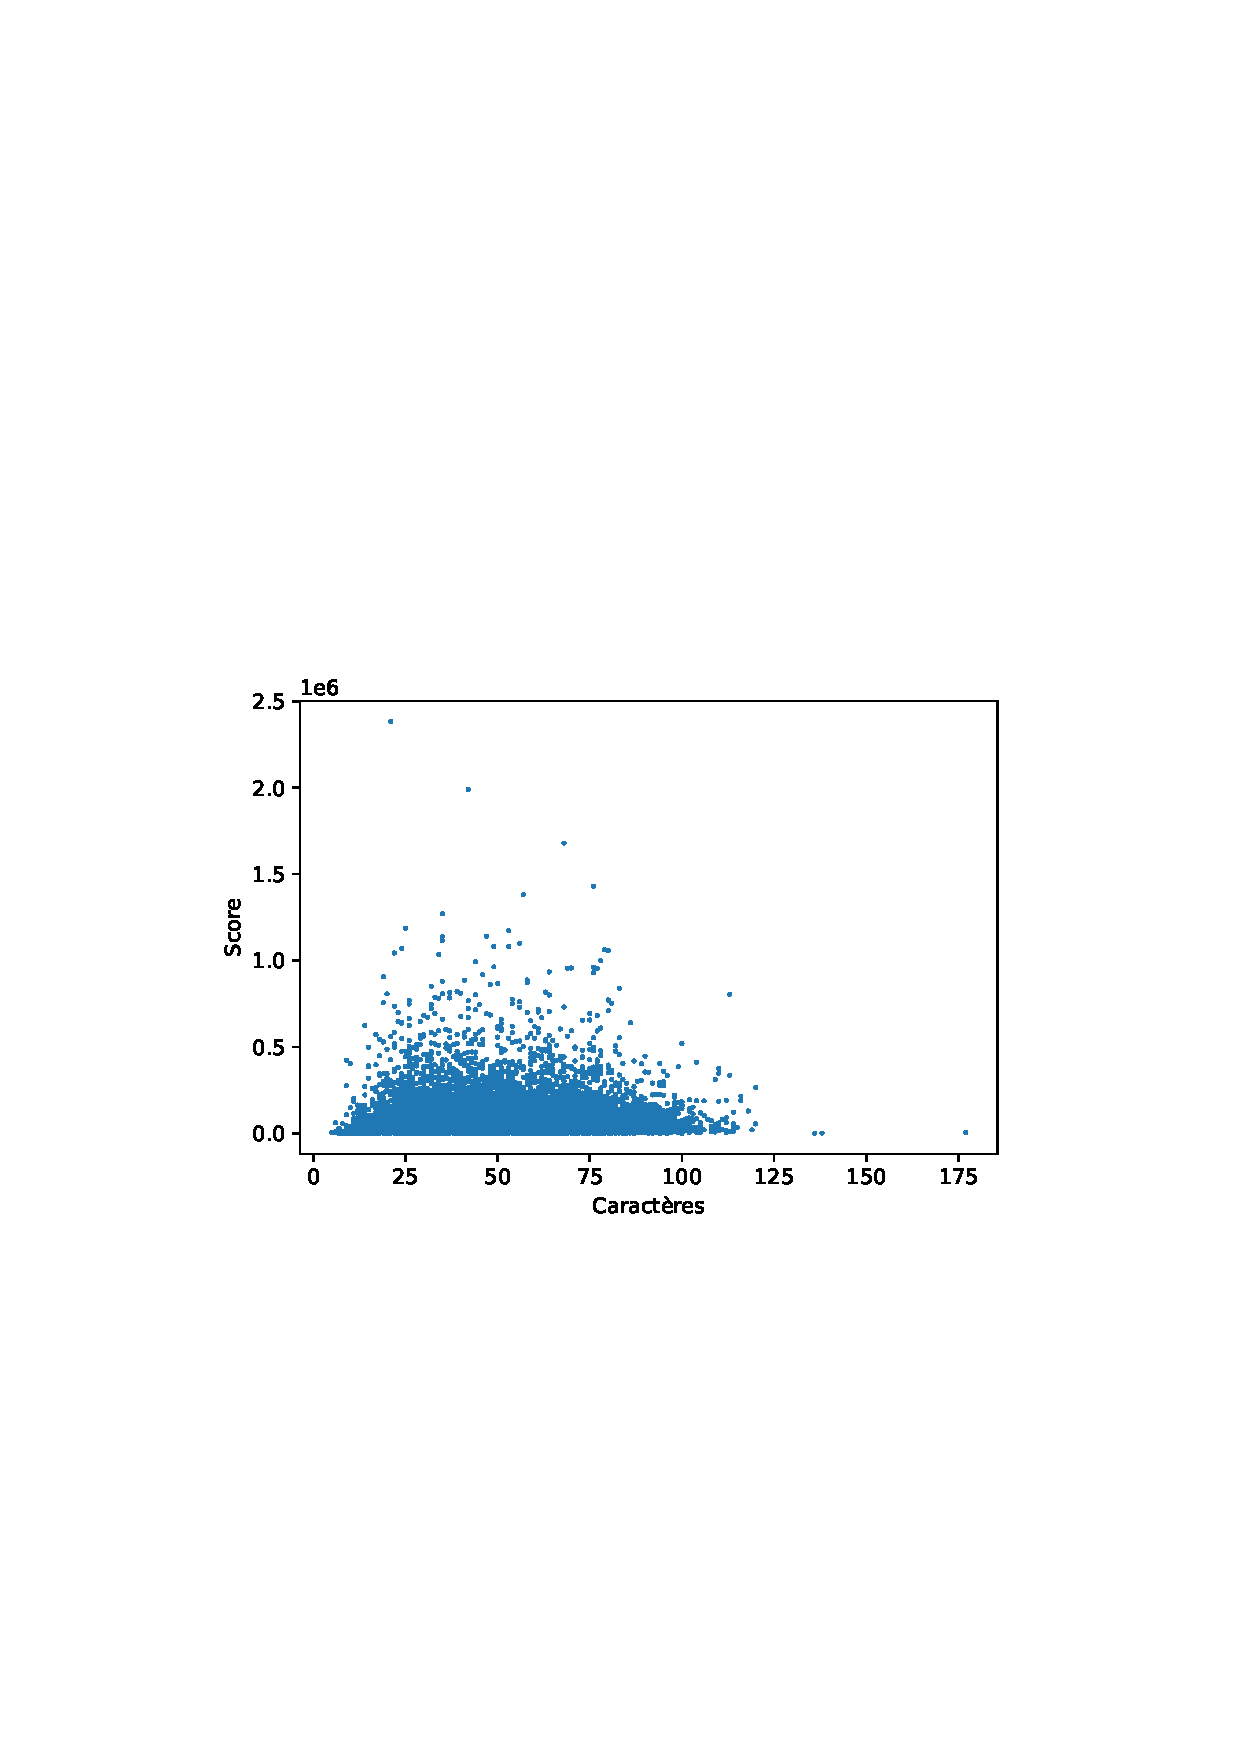
\includegraphics[width=0.6\textwidth]{dot_title_length_score_relation.png}
    \caption{Relation entre le score total et le nombre de caractères du titre}
    \label{fig:dot_title_length_score_relation}
    \end{figure}

D'après le graphique, il ne semble pas y avoir de corrélation forte ($r = 0.04$) entre le score d'un article et la longueur de son titre. De plus, la longueur du titre semble être standardisée pour ne pas dépasser entre 100 et 120 caractères environ, ce qui empêche une conclusion évidente.

\begin{figure}[H]
    \centering
    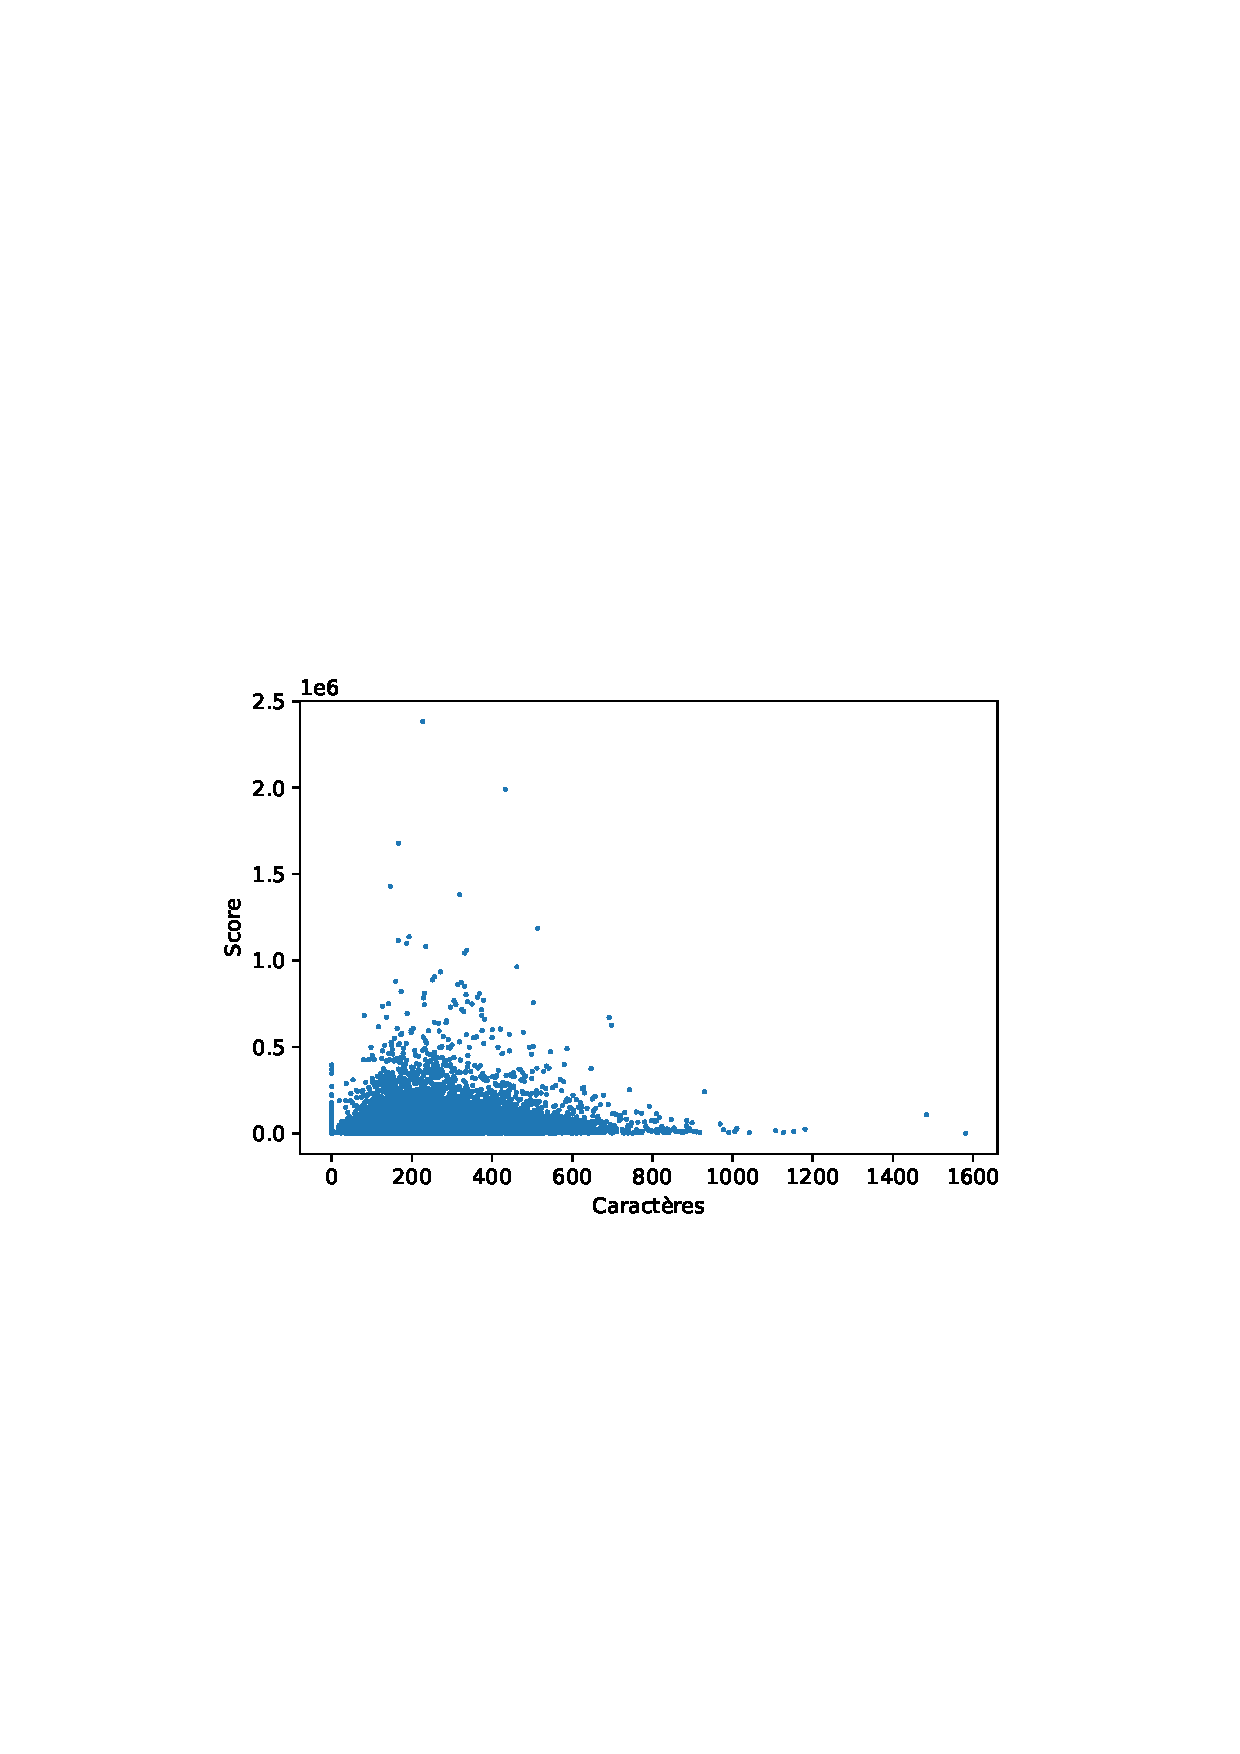
\includegraphics[width=0.6\textwidth]{dot_lead_length_score_relation.png}
    \caption{Relation entre le score total et le nombre de caractères du sous-titre}
    \label{fig:dot_lead_length_score_relation}
\end{figure}

Dans le cas des sous-titres, on ne trouve encore pas une corrélation élevée ($r = 0.06$) entre la longueur et le score.

On peut se demander si les articles qui provoquent un questionnement ou une sensation forte attirent l'attention des lecteurs. Une analyse simple peut se faire en comptant le pourcentage de titres avec un point d'interrogation ou un point d'exclamation.

\begin{figure}[H]
    \centering
    \includegraphics[width=0.6\textwidth]{pie_titres_avec_ponctuation.eps}
    \caption{Pourcentage de titres avec exclamation ou interrogation}
    \label{fig:pie_titres_avec_ponctuation}
    \end{figure}

\begin{figure}[H]
    \centering
    \includegraphics[width=0.6\textwidth]{pie_leads_avec_ponctuation.eps}
    \caption{Pourcentage de sous-titres avec exclamation ou interrogation}
    \label{fig:pie_leads_avec_ponctuation}
    \end{figure}

D'après l'analyse, les articles contenant dans le titre ou le sous-titre un point d'interrogation ou un point d'exclamation sont plutôt rares. Cependant, ces articles auront-ils en moyenne un score plus élevé?

\begin{figure}[H]
    \centering
    \includegraphics[width=0.6\textwidth]{bar_score_titres_ponctuation.eps}
    \caption{Scores moyens des titres avec ponctuation}
    \label{fig:bar_score_titres_ponctuation}
    \end{figure}

\begin{figure}[H]
    \centering
    \includegraphics[width=0.6\textwidth]{bar_score_leads_ponctuation.eps}
    \caption{Scores moyens des sous-titres avec ponctuation}
    \label{fig:bar_score_leads_ponctuation}
    \end{figure}
    

% score questionTitle.mean() : 76451.91332712023
% score normalTitle.mean() : 48080.41142320027
Bien que les titres ayant un point d'exclamation semblent performer un peu moins bien que les titres normaux, les titres ayant un point d'interrogation performent en moyenne 159\% mieux que les titres ordinaires. Il se peut que les titres contenant une question causent en effet une curiosité qui assure que le lecteur reste à la fin de l'article pour répondre à sa question. Il se peut aussi que les points d'exclamation indiquent le plus souvent un article sensationnel qui ne retienne pas aussi longtemps l'attention des lecteurs. Une relation semblable existe pour les sous-titres.


% Spécifier que les mots sont filtrés (prépositions, articles et filtrés pour que > 100 occurences)
Il serait interessant de savoir quel genre de mot retient l'attention des lecteurs. La figure \ref{fig:graph_bar_word_popular} montre la liste filtrée des mots présents dans les titres des articles ayant le meilleur score en moyenne:

\begin{figure}[H]
    \centering
    \includegraphics[width=0.9\textwidth]{graph_bar_word_popular.eps}
    \caption{Mots les plus populaire (moyenne du score) dans les titres}
    \label{fig:graph_bar_word_popular}
\end{figure}

Outre les mots ayant rapport aux actualités, on voit aussi que les titres contenant des médias [PHOTOS] ou [VIDÉO] sont populaires. Une analyse de type NLP plus approfondie sera nécessaire pour mieux comprendre l'impact du contenu du titre sur le score.

\subsubsection{Proportion d'articles sur mobile}

En matière de popularité absolue (score), les articles sur mobile sont plus performants en moyenne (figure \ref{fig:graph_pointagewebmobile}). Cependant, selon le nombre d'événements View à View 60, on observe que les utilisateurs mobiles sont plus enclins à cliquer sur un article et de le lire rapidement, comme le démontre la répartition des vues sur la figure \ref{fig:graph_mobile_views_repartition}. Le temps d'attention sur mobile est donc moins long. 

\begin{figure}[H]
\centering
\includegraphics[width=\textwidth]{gr002.png} 
\caption{Distribution du pointage - comparaison site web et mobile}
\label{fig:graph_pointagewebmobile}
\end{figure}


\begin{figure}[H]
\centering
\includegraphics[width=1.05\textwidth]{views.png} 
\caption{Quantité d'événements de vue (View) selon le journal de publication}
\label{fig:graph_mobile_views_repartition}
\end{figure}


% \subsection{Type de support visuel}
% Tel qu'anticipé, la plupart des articles possèdent un support visuel dont le type est majoritairement des photos, comme le montre la figure \ref{fig:graph_visual_repartition}. Il y a donc un déséquilibre de classe majeur pour la catégorie "photo" de l'attribut catégorique "visual.type". Cependant, il est intéressant d'observer sur la figure \ref{fig:graph_visual_score} que la présence de vidéos ou un type "slideshow" permet d'obtenir un score en moyenne plus élevé. Cette observation vient confirmer l'intuition que la présence de médias interactifs attire davantage les lecteurs.


% \begin{figure}
% \centering
% 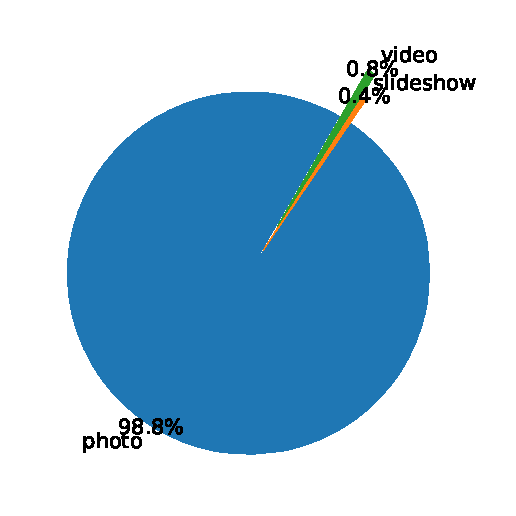
\includegraphics[width=0.6\textwidth]{graph_pie_visual_repartition.eps}
% \caption{Répartition des articles par type de support visuel}
% \label{fig:graph_visual_repartition}
% \end{figure}

% \begin{figure}
% \centering
% \includegraphics[width=0.8\textwidth]{graph_bar_visual_score.eps}
% \caption{Moyenne du score par type de support visuel}
% \label{fig:graph_visual_score}
% \end{figure}

\subsubsection{Catégories d'articles} \label{category-section}
Les données fournies permettent de catégoriser les articles à partir de la première partie de l'attribut \emph{slug} présent dans les métadonnées. En analysant les métadonnées, on observe que certaines informations permettant de mieux catégoriser un article donné. Par exemple, certains articles sont dans la classe \emph{actualité}, mais le slug contient \emph{actualites/justice-et-faits-divers/}, ce qui est plus spécifique. Cependant, un nettoyage des données plus approfondi reste nécessaire puisque la deuxième partie du slug n'est pas standardisé et contient du bruit. En effet, certains articles sont seuls dans leur catégorie, lorsque la deuxième partie du slug est considérée.

La figure \ref{fig:graph_category_repartition} présente la répartition de l'ensemble de tous les articles classés par catégorie. Les catégories représentant $<1\%$ ont été groupées dans \emph{Autre}. De plus, les articles d'actualité ont été regroupés dans une seule catégorie même si le type n'était pas écrit de la même façon (actualité pouvait être écrit au pluriel dans le slug).

Beaucoup d'articles sont classés dans les archives. Ces articles archivés n'apparaissent plus dans les données filtrés des 7 derniers mois. Lorsque les données des 7 derniers mois sont utilisées, près de la moitié des articles traitent de l'\emph{actualité}. Ce léger déséquilibre de classe peut avoir un impact sur la qualité de l'algorithme prédictif.

L'attribut \emph{channel} permet également de catégoriser plus précisément les articles. Par contre, la façon d'écrire le \emph{channel} n'est pas standardisée et un nettoyage des données est requis. Par exemple, \emph{Votre opinion}, \emph{Opinions} et \emph{Points de vue} sont tous des \emph{channel} différents.


\begin{figure}[H]
\centering
\includegraphics[width=0.95\textwidth]{graph_pie_category_repartition.eps}
\caption{Répartition des articles par catégorie}
\label{fig:graph_category_repartition}
\end{figure}

\subsubsection{Journée de publication}
Le groupe de travail a avancé que le score pouvait varier selon la journée à laquelle l'article était publié. Intuitivement, il était attendu que les pointages des articles publiés le weekend serait plus élevé que la semaine. Le graphique à la figure \ref{fig:graph_dayofweek} ne semble pas concluant, car les moyennes quotidiennes sont semblables. Une analyse plus précise, telle que des mesures de similarité/dissimilarité, sera nécessaire pour confirmer cette information.

\begin{figure}[h!]
\centering
\includegraphics[width=0.9\textwidth]{gr020.png}
\caption{Pointage des articles selon le jour (0 à 6 = lundi à dimanche)}
\label{fig:graph_dayofweek}
\end{figure}

\subsection{Cas problématiques}

\subsubsection{Informations manquantes}
Les données sont plutôt complètes puisque peu d'attributs sont manquants. Évidemment, la plupart des articles possèdent au moins un titre, un contenu et un auteur. Les attributs ayant quelques informations manquantes sont le \emph{channel}, le nom d'utilisateur Twitter et le \emph{sous-titre} des photos. Pour ne pas éliminer les articles avec des informations manquantes, la stratégie serait de remplir les attributs vides par une valeur catégorique (\emph{'Autre'}) ou une chaîne de caractères générique. L'autre stratégie serait d'éliminer l'attribut si celui-ci possède un trop grand nombre de lignes vides.

\subsubsection{Bruit dans les données}
L'attribut \emph{channel} est bruité puisque la classification de celui-ci n'est pas standardisée d'un journal à l'autre comme mentionné à la section \ref{category-section}. De plus, le nom des auteurs peut contenir le titre professionnel (ex: Professeur Émérite) ou contenir plusieurs noms d'auteurs (ex: Patrice Bergeron et Alexandre Robillard) en majuscule ou en minuscule. Particulièrement, le journal \emph{Le Droit} semble inclure le titre du journaliste ainsi que son adresse courriel dans le champ \emph{author}. Finalement, le contenu des chapitres devra être traité pour enlever toute traçe des balises HTML si une analyse de son contenu doit être effectuée.

\subsubsection{Déséquilibre de classes}
Certains attributs catégoriques présentent différents degrés de déséquilibre de classe. Principalement, un grand nombre d'articles sont peu ou pas vu et possèdent un score faible. Cela fait en sorte que la répartition du score n'est pas uniforme et qu'il y a un déséquilibre de classe.

% Analysez vos données et de leurs propriétés statistiques. 
% Portez attention autant aux valeurs normales qu’aux cas problématiques, comme la présence de bruit, le fléau de dimensionnalité, les
% informations manquantes, le déséquilibre des classes, les valeurs aberrantes, etc. Discutez de vos
% observations. L’objectif ici n’est pas de faire une grande liste de statistiques sur les données, mais
% d’en tirer des leçons pour guider la réalisation du projet. (3 points)

\section{Sélection des attributs}

Un grand nombre d'attributs peut avoir un impact sur la prédiction de la popularité (score) de l'article. La section suivante énumère les attributs choisis dans le cadre de l'étude.









\subsection{Attributs stylistiques et linguistique}
\textbf{title} : Un titre accrocheur permet d'obtenir davantage de vues. Cet attribut permettra d'analyser les mots et la présence de ponctuation du titre qui permettent de maximiser le score. Le titre sera stocké comme une chaîne de caractères, mais d'autres attributs pourraient en être dérivés.
\textbf{visual} Plus particulièrement, dans l'objet il sera intéressant d'extraire les chaînes de caractère du \textbf{type} et du \textbf{caption}. Le \textbf{visual.type} permettra de catégoriser les articles à savoir s'ils contiennent des vidéos, des photos ou un type slideshow. Le \textbf{visual.caption} permettra d'en analyser le contenu de la même façon que l'attribut \textbf{title}.

\textbf{chapters} : L'attribut chapters permettra d'extraire le contenu du texte (\textbf{chapters.text}) ainsi que le type de paragraphe (\textbf{chapters.type}). Ainsi le type chapitre pourra être compté par article pour connaître le nombre de paragraphes de l'article ainsi que le nombre de paragraphes contenant des photos. L'hypothèse étant qu'un article ayant d'avantage de photos dans le texte sera lu plus longtemps et fera augmenter le score.

\subsection{Attributs sociaux}

\textbf{authors} : Comme la plupart des articles n'ont qu'un auteur \cite{rapport12019}, le premier auteur de la liste sera sélectionné. Logiquement, un chroniqueur connu dans la région aura une masse critique de lecteurs qui voudront le lire hebdomadairement (ex : les chroniques de Patrick Lagacé à LaPresse sont lus davantage en partie grâce à sa renommée). L'attribut authors est une chaîne de caractères.

\textbf{authors.twitter} : Twitter n'est pas le réseau social le plus utilisé au Québec. Néanmoins, l'hypothèse posée est qu'un auteur qui possède beaucoup de \emph{suiveurs} sur twitter risque de voirs ses articles être plus populaires. Le nom d'utilisateur Twitter est une chaîne de caractère.


\subsection{Méta-Attributs}

\textbf{product}: L'attribut \textbf{product} représente l'un des 6 journaux dont l'article a été vu. Cet attribut permettra de déterminer si certains journaux sont plus populaires. Par exemple, \emph{Le Soleil} dessert la grande région de Québec qui possède un bassin de lecteurs plus important que \emph{Le Nouvelliste} de Trois-Rivières.

\textbf{publicationDate} : Certaines périodes, comme l'été, sont moins riches en actualités; l'hypothèse peut être faite que les journaux sont moins lus selon la période de l'année. Également, la population active consomme généralement les journaux à certaines périodes de la journée (matin, midi et soir). Donc un article publié au bon moment risque de maximiser sa popularité.

\textbf{slug} : Le slug contient la catégorie dans laquelle l'article a été classifié dans le journal. La popularité d'un article peut varier selon la catégorie et il est important pour l'aide à la rédaction de tenir compte de la catégorie de l'article. Cependant, beaucoup de vieux articles sont dans la section archives. Pour contrer ceci, un nettoyage des données pourra être fait pour reclassifier ces articles à l'aide de l'attribut \textbf{channel} qui donne le sujet spécifique de l'article.

\textbf{channel} : Le \emph{channel} est une description de l'article à l'aide d'un mot-clé (analogue aux hashtags sur twitter). Comme mentionné dans la description de l'attribut \emph{slug}, ceux-ci pourront servir au nettoyage ou à la reclassification du slug. Par contre, le \emph{channel} est très bruité et un regroupement des catégories sera requis pour réduire le fléau de la dimensionnalité.

% \textbf{hasMobile}: L'attribut hasMobile a été dérivé par notre équipe à partir des données. Cet attribut booléen indique \emph{Vrai} si les métadonnés montrent que l'article a été publié dans au moins une section mobile et \emph{Faux} si l'article n'a pas été publié sur une plateforme mobile. L'hypothèse étant que les articles publiés sur mobile ont davantage de vues (\emph{View}), mais sont lus moins longtemps (\emph{View60}).



% Prévoyez les attributs que vous allez utiliser pour votre algorithme de traitement de données. Il y a
% une immense variété d’attributs qui peuvent être obtenus de ces données, incluant des attributs
% linguistiques (les mots utilisés dans l’article, les adverbes, etc.), des attributs numériques (la longueur
% de l’article en mots, en paragraphes, le nombre de photos, le niveau de difficulté du texte, etc.), des
% attributs stylistiques (le contenu du titre, le contenu des photos, l’utilisation de citations, etc.), des
% attributs sociaux (l’inclusion de tweets, de vidéos YouTube, etc.), et des méta-attributs (le sujet de
% l’article, l’heure de publication, etc.). Vous devez prévoir les premiers attributs sur lesquels vous allez
\section{Traitement des données}

%% La section parlant d'algorithme est à réviser !
Le but principal du projet est de prédire un score à partir d'attributs sélectionnés. Plusieurs algorithmes d'apprentissage machine permettent de résoudre ce type de problème. Dans le cadre du cours, deux algorithmes de classification seront évalués : les arbres de décision et le classificateur naïf de Bayes. Chacune des méthodes offre des avantages et désavantages qui seront approfondis par leur application à l'ensemble des données disponibles.

Dans un premier temps, l'arbre de décision offre une vision de la classification stricte qui peut être comprise par l'usager.  Comme l'algorithme va du cas général au particulier (top-down) tout en prenant la meilleure décision à chaque moment (greedy), le processus de l'arbre de décision peut facilement être suivi et compris. Cette technique présente aussi la capacité de distribuer les calculs et d'éviter le surapprentissage. Les arbres de décision demeurent cependant sensibles au fléau de dimensionnalité. Un arbre de régression semble être adapté à ce problème de classification numérique du score. Ainsi, plusieurs sous-catégories d'arbres décision peuvent être explorées telles que les forêts aléatoires et les \emph{boosted trees}. Ces algorithmes sont accessibles dans des librairies telles que \emph{scikit-learn} ou \emph{XGboost}.

En comparaison, le classificateur naïf de Bayes propose une approche basée sur la probabilité d'identifier une classe grâce à ses attributs. Cet algorithme nécessite une quantité massive de données afin d'observer les bonnes probabilités des attributs dans chaque classe et les valeurs rares des. Ce classificateur évite le fléau de la dimensionnalité, offre des résultats facilement interprétables, et donne généralement de bons résultats.


Enfin, pour un problème possédant un grand nombre de données et plusieurs attributs, le réseau de neurones est souvent l'algorithme de choix. Vu la disponibilité de librairies Python, telles que \emph{Tensorflow}, pour implanter un réseau de neurones, cette avenue sera aussi explorée par notre équipe afin de comparer les résulats avec les deux approches précédentes.

% Mentionner que certains articles semblent être virals donc il est anticipé qu'il faudra regrouper le score en certains intervalles.


Vu la grande quantité de données et la limitation de mémoire des ordinateurs disponibles, les algorithmes pourront prendre trop de temps de traitement. Une stratégie palliative serait de prendre un échantillon aléatoire des données (fonction \emph{sample} dans la librairie Pandas dans Python) entrant en mémoire. Cet échantillon serait utilisé pour déterminer les hyperparamètres finaux de l'algorithme, qui pourra alors être entraîné sur la population complète des données.

%% Trouver une meilleure méthode d'optimisation des algo.. Par expérience personnelle souvent on peut pas faire des miracles sans avoir des bonnes données. Le mieux qu'on peut faire c'est d'optimiser les hyperparameters.
Une attention particulière sera également portée sur la sélection des hyperparamètres de l'algorithme afin d'éviter le fléau du surapprentissage.

L'optimisation des algorithmes peut être limitée par la qualité et la quantité des données qui lui sont fournies. Comme mentionné, les données étiquetées sont disponibles que pour les 7 derniers mois de vues. Puisque les autres articles non étiquetés contiennent de l'information permettant d'améliorer la prédiction, une façon d'étiqueter ces données devra être déterminée. Puisqu'il est impossible d'étiqueter les valeurs par un humain, un algorithme d'apprentissage semi-supervisé doit être utilisé pour prédire les étiquettes manquantes. Puisque la précision du score est relativement importante, un algorithme robuste tel qu'un classificateur entraîné avec des hyperparamètres différents à chaque itération pourrait être utilisé. 


% Prévoyez comment vous allez traiter les données d’un point de vue pratique. C’est-à-dire
% premièrement les algorithmes que vous allez implémenter, mais aussi l’optimisation de ceux-ci afin
% de pouvoir traiter la quantité massive de données disponible pour ce projet de manière efficace. (2
% points).

% Checklist
% Algo à utiliser : arbre ou réseau
% Comment utiliser les données non-étiqueté
% Comment traiter l'ensemble des données (DASK ou échantillonner)
% Expliquer comment traiter les articles ayant plus de temps depuis la publication en ligne (en analysant les clicks dans le temps)
% Expliquer comment traiter les catégories d'articles ou channels qui sont populaires mais petit en nombre (genre jeux olympiques) => FAute de moyen on voudra mettre dans une catégorie "autre"

\section{Méthodologie de test}
% Discutez également de la procédure de tests que vous envisagez. Vous ne pouvez pas tester votre
% système avec la liste d’identifiants d’évaluation, car vous n’avez pas les résultats réels pour ces
% articles. Vous devez donc prévoir votre propre procédure de tests afin de savoir si chaque variation
% que vous implémentez pour votre solution améliore ou non vos prédictions, et ainsi guider votre
% travail de développement. (2 point)

La méthode de validation croisée de type \emph{K-Fold} consiste à séparer les données en partitions égales et en faire l'entrainement sur une portion des partitions, sauf une, qui sert de validation. Cette portion de partition de validation croisée est changeante à chaque itération. L'utilisation de cette méthode permettra d'estimer l'efficacité de l'algorithme et de ses \emph{hyperparamètres} sans passer par le sous-ensemble de test. Les différents algorithmes implantés seront comparés sur la base de l'erreur de prédiction du score sur les partitions de \emph{validation croisée}. La portion de données contenues dans la partition de validation sera fixée à $20\%$. La séparation des données d'entraînement et de test sera donc de 80/20.




% Le rapport pour cette partie devrait être d’environ 10 pages et est dû le 24 février 2021

\bibliographystyle{plain}
\bibliography{references}
\end{document}
